\documentclass{article}

\usepackage[landscape, twocolumn, top=1in, bottom=0.8in, left=0.4in, right=0.4in]{geometry}

% font
\usepackage{fontspec}
\setmainfont{Georgia}[
  Path=./fonts/,
  Extension = .ttf,
  UprightFont=*-Regular,
  BoldFont=*-Bold,
  ItalicFont=*-Italic,
  BoldItalicFont=*-BoldItalic
]
\setsansfont{Metropolis}[
  Path=./fonts/,
  Extension = .ttf,
  UprightFont=*-Medium,
  BoldFont=*-Bold,
]

% utility packages
\usepackage{amsmath, amsthm, amssymb}
\usepackage{mathtools}
\usepackage[many]{tcolorbox}
\usepackage{xcolor}
\usepackage{titlesec}
\usepackage{titling}
\usepackage{enumitem}   
\usepackage{fancyhdr,lipsum}
\usepackage{float}
\usepackage{tikz}
\usepackage{enumitem}

% change font size
\usepackage[fontsize=7pt]{fontsize}

% header line
% \fancyhead[L]{\textit{06/15/2022}}
\fancyhead[R]{\textit{Duc Nguyen}}
\fancyhead[C]{{Tropical Algebra}}
\renewcommand{\headrulewidth}{0.4pt}
\renewcommand{\footrulewidth}{0pt}
\pagestyle{fancy}

% disable bibliography chapter title
% \usepackage{natbib}
% \renewcommand{\bibsection}{}

\definecolor{grey}{rgb}{0.5,0.5,0.5}
\definecolor{lightgrey}{rgb}{0.8,0.8,0.8}
\definecolor{darkgrey}{rgb}{0.3,0.3,0.3}
\definecolor{orange}{rgb}{0.94, 0.55, 0.294}
\definecolor{pink}{rgb}{0.94, 0.29, 0.7}
\definecolor{yellow}{rgb}{1, 0.749, 0}
\definecolor{green}{rgb}{0.235,0.702,0.443}
\newcommand{\chapfnt}{\fontsize{16}{19}}
\newcommand{\secfnt}{\fontsize{14}{8}}
\newcommand{\ssecfnt}{\fontsize{11}{0}}

\renewcommand{\hline}{\noindent\makebox[\linewidth]{\rule{12cm}{1pt}}}

\titleformat{\chapter}[display]
{\normalfont\chapfnt\bfseries}{\chaptertitlename\ \thechapter}{20pt}{\chapfnt}

\titleformat{\section}
{\normalfont\sffamily\secfnt\bfseries}{\thesection}{}{}

\titleformat{\subsection}
{\normalfont\sffamily\ssecfnt\mdseries}{\thesubsection}{}{}

\titleformat{\subsubsection}
{\normalfont\sffamily\fontsize{9}{0}\mdseries\color{grey}}{\thesubsection}{}{}

\titlespacing*{\chapter} {0pt}{50pt}{40pt}
\titlespacing*{\section} {0pt}{0pt}{8pt}
\titlespacing*{\subsection} {0pt}{12pt}{8pt}

\linespread{1.3}

\newtcbtheorem[auto counter,number within=section]{theorem}%
{Theorem}{
    fonttitle=\upshape, 
    fontupper=\upshape,
    boxrule=0pt,
    leftrule=3pt,
    arc=0pt,auto outer arc,
    colback=white,
    colframe=orange,
    colbacktitle=white,
    coltitle=orange,
    oversize,
    enlarge top by=1mm,
    enlarge bottom by=1mm,
    enhanced jigsaw,
    interior hidden, 
    before skip=12pt,
    overlay={
      \draw[line width=1.5pt,orange] (frame.north west) -- (frame.south west);
    }, 
    frame hidden}{theorem}
    
\newtcbtheorem[]{exercise}%
{Exercise}{
      theorem name,
    fonttitle=\upshape, 
    fontupper=\upshape,
    boxrule=0pt,
    leftrule=3pt,
    arc=0pt,auto outer arc,
    colback=white,
    colframe=pink,
    colbacktitle=white,
    coltitle=pink,
    oversize,
    enlarge top by=1mm,
    enlarge bottom by=1mm,
    enhanced jigsaw,
    interior hidden, 
    before skip=12pt,
    after skip=0pt,
    overlay={
      \draw[line width=1.5pt,pink] (frame.north west) -- (frame.south west);
    }, 
    frame hidden}{exercise}

\newtcbtheorem[auto counter,number within=section]{lemma}%
{Lemma}{
    fonttitle=\upshape, 
    fontupper=\upshape,
    boxrule=1pt,
    toprule=0pt,
    leftrule=3pt,
    arc=0pt,auto outer arc,
    colback=white,
    colframe=orange,
    colbacktitle=white,
    coltitle=orange,
    oversize,
    enlarge top by=1mm,
    enlarge bottom by=1mm,
    enhanced jigsaw,
    interior hidden, 
    before skip=12pt,
    after skip=0pt,
    overlay={
      \draw[line width=1.5pt,orange] (frame.north west) -- (frame.south west);
    }, 
    frame hidden}{lemma}
    
\newtcbtheorem[auto counter,number within=section]{example}%
{Example}{
    fonttitle=\upshape, 
    fontupper=\upshape,
    boxrule=1pt,
    toprule=0pt,
    leftrule=3pt,
    arc=0pt,auto outer arc,
    colback=white,
    colframe=green,
    colbacktitle=white,
    coltitle=green,
    oversize,
    enlarge top by=1mm,
    enlarge bottom by=1mm,
    enhanced jigsaw,
    interior hidden, 
    before skip=12pt,
    overlay={
      \draw[line width=1.5pt,green] (frame.north west) -- (frame.south west);
    }, 
    frame hidden}{example}
    
\newtcbtheorem[]{important}%
{Wichtig}{
    fonttitle=\upshape, 
    fontupper=\upshape,
    boxrule=0pt,
    leftrule=3pt,
    arc=0pt,auto outer arc,
    colback=white,
    colframe=pink,
    colbacktitle=white,
    coltitle=pink,
    oversize,
    enlarge top by=1mm,
    enlarge bottom by=1mm,
    enhanced jigsaw,
    interior hidden, 
    before skip=12pt,
    overlay={
      \draw[line width=1.5pt,pink] (frame.north west) -- (frame.south west);
    }, 
    frame hidden}{important}
    
\renewcommand{\baselinestretch}{1.4} 
\makeatletter
\let\old@rule\@rule
\def\@rule[#1]#2#3{\textcolor{lightgrey}{\old@rule[#1]{#2}{#3}}}
\makeatother


\begin{document}

\section*{Tropical Algebra}

\subsection*{I. Tropical Arithmetic}

\begin{itemize}
	\item \textbf{\emph{Tropical semiring}} \( (\bar{\mathbb{R}}, \oplus, \odot) \) is the set \( \bar{\mathbb{R}} = \mathbb{R} \cup \left\{  \infty \right\}\) with 
	\begin{gather*}
		y \oplus x = \min\left\{ x,y \right\} \quad \text{and} \quad x \odot y = x + y \qquad x,y \in \bar{\mathbb{R}} 
	\end{gather*}
	For example:
		\begin{align*}
			4 \oplus 5 = 4, \quad4 \odot 5 = 9, \quad (-100) \oplus (-10) = -100, \quad x= 0 \odot x \quad \forall x \in \mathbb{R}
		\end{align*}

		\begin{exercise}{Warmup}{}
			Calculate (i) \( 10 \oplus -5 \), (ii) \( 8 \odot -4 \), (iii) \( 10 \oplus \infty \), and (iv) \( 4^{\odot 5} \).
		\end{exercise}

		\begin{exercise}{What is the additive and multiplicative neutral element?}{}
		Find an \( x \in \mathbb{R} \cup \left\{ \infty \right\} \) such that \( y = y \oplus x \) for all \( y \in \mathbb{R} \).

		Find an \( x \in \mathbb{R} \) such that \( y = y \odot x \) for all \( y \in \mathbb{R} \).
		\end{exercise}
	
		\begin{exercise}{What is the division? How about subtraction?}{}
		Find an \( x \in \mathbb{R} \) such that \( 10 = x \odot 3 \). Can we always do this?
		
		Can we find \( x \in \mathbb{R} \) such that \( 17 = 10 \oplus x \)?
		\end{exercise}

	\item Matrix-Vector operations: \( \oplus \) and \( \odot \) operate in \( \bar{\mathbb{R}}^{n \times n} \) as we would expect it
	\begin{align*}
		\begin{bmatrix}
			4 \\ 2
		\end{bmatrix}
		\oplus
		\begin{bmatrix}
			2 \\ 5
		\end{bmatrix}
		= 
		\begin{bmatrix}
			\min\left\{ 4,2 \right\} \\
			\min \left\{ 2,5 \right\}
		\end{bmatrix} = \begin{bmatrix}
			2 \\ 2
		\end{bmatrix}, \quad 
		42 \odot 
		\begin{bmatrix}
			3 \\ 2
		\end{bmatrix} = \begin{bmatrix}
			45 \\ 44
		\end{bmatrix}, \quad \begin{bmatrix}
			2 & 3 \\
			5 & 11
		\end{bmatrix} \odot
		\begin{bmatrix}
			4 \\ 0
		\end{bmatrix} =
		\begin{bmatrix}
			3 \\ 9
		\end{bmatrix} 
	\end{align*}

	\begin{figure}[H]
		\centering
		\begin{subfigure}{.25\textwidth}
			\centering
			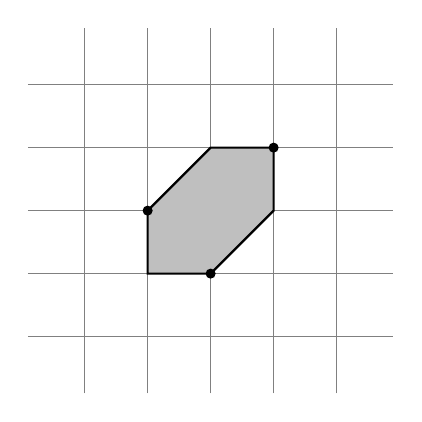
\begin{tikzpicture}[scale=0.8]
				\draw[step=1cm,gray,very thin] (-2.9,-2.9) grid (2.9,2.9);
	
				\filldraw[color=black, fill=black!25, thick] (-1, 0) -- (-1,-1) -- (0,-1) -- (1,0) -- (1,1) -- (0, 1) -- (-1, 0);
	
				\filldraw[black] (-1,0) circle (2pt);
				\filldraw[black] (0,-1) circle (2pt);
				\filldraw[black] (1,1) circle (2pt);
			\end{tikzpicture}
			\caption{The tropical image of a \( 3 \times 3 \)-matrix in \( \mathbb{R}^3 / \mathbf{1} \mathbb{R} \)}
		\end{subfigure}%
		\begin{subfigure}{.25\textwidth}
			\centering
			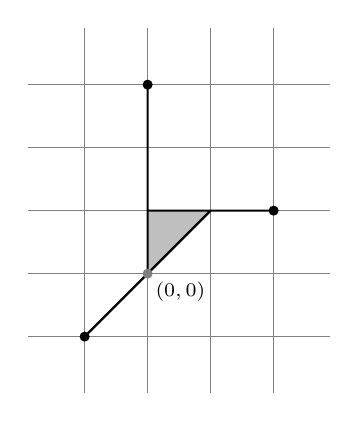
\begin{tikzpicture}[scale=0.8]
				\draw[step=1cm,gray,very thin] (-1.9,-1.9) grid (2.9,3.9);
	
				\draw[color=black, fill=black!25, thick] (-1,-1) -- (0,0) -- (0,3) -- (0,1) -- (2,1) -- (1,1) -- (0,0);
	
				\filldraw[black] (-1,-1) circle (2pt);
				\filldraw[black] (0,3) circle (2pt);
				\filldraw[black] (2,1) circle (2pt);
	
				\filldraw[gray] (0,0) circle (2pt);
				\node[anchor=north west] at (0,0) {$(0,0)$};
			\end{tikzpicture}
			\caption{A tropical triangle in \( \mathbb{R}^3 / \mathbf{1} \mathbb{R} \)}
		\end{subfigure}

		
	\end{figure}
\end{itemize}

\subsection*{II. Tropical Linear Algebra}

\subsubsection*{A. Tropical Matrices and Shortest Path}

\begin{itemize}
	 \item Tropical arithmetic occurs naturally in discrete math; for example

		\begin{theorem*}{Shortest Path \cite[Prop. 7.9]{inv2nonlinearalgebra}}{}
			Let \( D_G  \) be the adjacency matrix of a directed graph \( G \) which has only non-negative edges and contains no loops.
			Then, the length of the shortest path from node \( i \) to \( j \) is given by row \( i \) and column \( j \) of the matrix 
			\begin{align*}
				D_G^{\odot(n-1)} = D_G \odot \cdots \odot D_G.
			\end{align*}
		\end{theorem*}

		\begin{proof}
			See blackboard.
		\end{proof}
		
		\begin{example*}{}{}
			\begin{figure}[H]
				\centering
				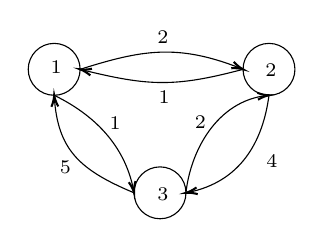
\begin{tikzpicture}[x=0.75pt,y=0.75pt,yscale=-0.5,xscale=0.5]
%uncomment if require: \path (0,318); %set diagram left start at 0, and has height of 318

%Shape: Circle [id:dp8552406885330566] 
\draw   (100,155) .. controls (100,141.19) and (111.19,130) .. (125,130) .. controls (138.81,130) and (150,141.19) .. (150,155) .. controls (150,168.81) and (138.81,180) .. (125,180) .. controls (111.19,180) and (100,168.81) .. (100,155) -- cycle ;
%Shape: Circle [id:dp09770625656490761] 
\draw   (307,155) .. controls (307,141.19) and (318.19,130) .. (332,130) .. controls (345.81,130) and (357,141.19) .. (357,155) .. controls (357,168.81) and (345.81,180) .. (332,180) .. controls (318.19,180) and (307,168.81) .. (307,155) -- cycle ;
%Shape: Circle [id:dp20108922600222412] 
\draw   (202,274) .. controls (202,260.19) and (213.19,249) .. (227,249) .. controls (240.81,249) and (252,260.19) .. (252,274) .. controls (252,287.81) and (240.81,299) .. (227,299) .. controls (213.19,299) and (202,287.81) .. (202,274) -- cycle ;
%Curve Lines [id:da03416611292826599] 
\draw    (150,155) .. controls (208.71,136.56) and (243.65,129.54) .. (306.06,154.62) ;
\draw [shift={(307,155)}, rotate = 202.06] [color={rgb, 255:red, 0; green, 0; blue, 0 }  ][line width=0.75]    (10.93,-3.29) .. controls (6.95,-1.4) and (3.31,-0.3) .. (0,0) .. controls (3.31,0.3) and (6.95,1.4) .. (10.93,3.29)   ;
%Curve Lines [id:da09658173369640033] 
\draw    (307,155) .. controls (241.33,172.38) and (216.25,171.48) .. (150.99,155.25) ;
\draw [shift={(150,155)}, rotate = 14.01] [color={rgb, 255:red, 0; green, 0; blue, 0 }  ][line width=0.75]    (10.93,-3.29) .. controls (6.95,-1.4) and (3.31,-0.3) .. (0,0) .. controls (3.31,0.3) and (6.95,1.4) .. (10.93,3.29)   ;
%Curve Lines [id:da3395837262637085] 
\draw    (332,180) .. controls (326.06,225.01) and (304.44,263.69) .. (253.55,273.71) ;
\draw [shift={(252,274)}, rotate = 349.61] [color={rgb, 255:red, 0; green, 0; blue, 0 }  ][line width=0.75]    (10.93,-3.29) .. controls (6.95,-1.4) and (3.31,-0.3) .. (0,0) .. controls (3.31,0.3) and (6.95,1.4) .. (10.93,3.29)   ;
%Curve Lines [id:da5148363316884303] 
\draw    (252,274) .. controls (255.96,235.85) and (280.5,185.49) .. (330.48,180.15) ;
\draw [shift={(332,180)}, rotate = 174.99] [color={rgb, 255:red, 0; green, 0; blue, 0 }  ][line width=0.75]    (10.93,-3.29) .. controls (6.95,-1.4) and (3.31,-0.3) .. (0,0) .. controls (3.31,0.3) and (6.95,1.4) .. (10.93,3.29)   ;
%Curve Lines [id:da9847848128429115] 
\draw    (202,274) .. controls (148.54,251.69) and (128.4,231.87) .. (125.1,181.53) ;
\draw [shift={(125,180)}, rotate = 86.66] [color={rgb, 255:red, 0; green, 0; blue, 0 }  ][line width=0.75]    (10.93,-3.29) .. controls (6.95,-1.4) and (3.31,-0.3) .. (0,0) .. controls (3.31,0.3) and (6.95,1.4) .. (10.93,3.29)   ;
%Curve Lines [id:da7368989634069993] 
\draw    (125,180) .. controls (168.34,201.15) and (194.22,232.51) .. (201.67,272.18) ;
\draw [shift={(202,274)}, rotate = 260.2] [color={rgb, 255:red, 0; green, 0; blue, 0 }  ][line width=0.75]    (10.93,-3.29) .. controls (6.95,-1.4) and (3.31,-0.3) .. (0,0) .. controls (3.31,0.3) and (6.95,1.4) .. (10.93,3.29)   ;

% Text Node
\draw (119,144.4) node [anchor=north west][inner sep=0.75pt]    {$1$};
% Text Node
\draw (326,147.4) node [anchor=north west][inner sep=0.75pt]    {$2$};
% Text Node
\draw (222,266.4) node [anchor=north west][inner sep=0.75pt]    {$3$};
% Text Node
\draw (222,115.4) node [anchor=north west][inner sep=0.75pt]    {$2$};
% Text Node
\draw (223,173.4) node [anchor=north west][inner sep=0.75pt]    {$1$};
% Text Node
\draw (327,235.4) node [anchor=north west][inner sep=0.75pt]    {$4$};
% Text Node
\draw (258,197.4) node [anchor=north west][inner sep=0.75pt]    {$2$};
% Text Node
\draw (128,240.4) node [anchor=north west][inner sep=0.75pt]    {$5$};
% Text Node
\draw (176,198.4) node [anchor=north west][inner sep=0.75pt]    {$1$};
\end{tikzpicture}
			\end{figure}
			$$
				D_G = \begin{bmatrix}
					0 & 2 & 1 \\
					1 & 0 & 4 \\
					5 & 2 & 0
				\end{bmatrix} \quad \text{and} \quad D_G^{\odot 2} = \begin{bmatrix}
					0 & 2 &1 \\ 1 & 0 & 2 \\ 3 & 2 & 0
				\end{bmatrix}.
			$$

			Row \( 3 \) and column \( 1 \) of \(  D_G^{\odot 2} \) yields that the shortest path from node \( 3 \) to \( 1 \) has length \( 3 \) (consider path \( 3 \leadsto 2 \leadsto 1 \) which is shorter that \( 3 \leadsto 1 \)). 
		\end{example*}

		\begin{exercise}{Find the length of each shortest path.}{}
			\begin{figure}[H]
				\centering
				\input{tikz/shortest-path-exercise.tikz}
			\end{figure}
		\end{exercise}

		\item Theorem fails for graphs with loops; however, the \textbf{\textit{Kleene plus}} \( 	D_G^+ = D_G \oplus D_G^{\odot 2} \oplus ... \oplus D_G^{\odot n} \) generalizes the Shortest Path Theorem to graphs with \emph{negative} edge lengths and \emph{loops} \cite[Exercise 1.9 (5)]{MaclaganSturmfels}
	\end{itemize}
 	
	\subsubsection*{B. Determinant and the Assignment Problem}
\begin{itemize}
	\item The \textbf{\emph{tropical determinant}} of an \( n \times n \)-matrix \( X = (x_{ij}) \) is defined as 
	\begin{align*}
		\mathrm{tropdet}(X) = \bigoplus_{\pi \in S_n} x_{1 \pi(1)} \odot x_{2 \pi(2)} \odot \cdots \odot x_{n \pi(n)},
	\end{align*}
	where \( S_n = \left\{ \pi : \text{\( \pi\) is a permutation of } \left\{ 1,2,...,n \right\}\right\} \)
	\begin{theorem*}{Assignment Problem  \cite[Prop. 7.10]{inv2nonlinearalgebra}}{}
		The optimal cost of the assignment problem is given by the tropical determinant.
	\end{theorem*}
	\begin{proof}
		Follows directly from definition.
	\end{proof}

	\begin{example*}{}{}
		\( \mathrm{tropdet} \begin{bmatrix}
			1 & 5 & \mathbf{0} \\
			\mathbf{2} & 7 & 4 \\
			0 & \mathbf{3} & 2
		\end{bmatrix} = 0 \odot 2 \odot 3 = 5 \)
	\end{example*}

	\begin{exercise*}{Calculate the tropical determinant.}{}
		\( \mathrm{tropdet} \begin{bmatrix}
			0 & 4 & 1 \\
			1 & 8 & 6 \\
			1 & 2 & 0
		\end{bmatrix} \)
	\end{exercise*}

\end{itemize}

\subsubsection*{C. Eigenvalues and Cycle Lengths}
\begin{itemize}
	\item An \textbf{\textit{eigenvalue}} \( \lambda \in \mathbb{R}  \) of \( A \in \bar{\mathbb{R}}^{n \times n} \) is a scalar that satisfies 
	\begin{align*}
		A \odot v = \lambda \odot v\quad \text{for some \( v \in \mathbb{R}^n \)}
	\end{align*}
 
	\begin{theorem*}{Square matrices have exactly one eigenvalue  \cite[Thm. 7.11]{inv2nonlinearalgebra}}{}
		Let \( A \) be an \( n \times n \)-matrix whose graph \( G(A) \) is strongly connected. Then, \( A \) has \emph{precisely} one eigenvalue, denoted \( \lambda(A) \). The eigenvalue \( \lambda(A) \) equals the minimum of normalized length over all directed cycles in \( G(A) \).
	\end{theorem*}

	\begin{proof}
		Use the {\textit{Kleene plus}}.
	\end{proof}

	\begin{example*}{}{}
		\input{tikz/eigenvalue-graph.tikz}

		Consider the \( 1 \)-cycle \( 2 \leadsto 2 \). It has normalized length \( \frac{7}{1} = 7 \).

		Consider the \( 2 \)-cycle \( 1 \leadsto 2 \leadsto 1 \). It has normalized length \( \frac{5 + 2}{2} = 3.5 \).

		Consider the \( 2 \)-cycle \( 1 \leadsto 3 \leadsto 1 \). It has normalized length \( \frac{0 + 0}{2} = 0 \). In fact, \( \lambda(A) = 0 \).
	\end{example*}

	\begin{exercise*}{Calculate the eigenvalue}{}
		\( A = \begin{bmatrix}
			3 & 1 \\
			1 & 4
		\end{bmatrix} \), \, \(  B = \begin{bmatrix}
			3 & 4 & 4 \\
			4 & 3 & 4 \\
			4 & 4 & 3
		\end{bmatrix} \), \, \( C =  \begin{bmatrix}
			3 & 1 & 4 \\
			1 & 3 & 2 \\
			4 & 4 & 3
		\end{bmatrix}\)
	\end{exercise*}
\end{itemize}

\subsection*{C. Literature}
\bibliographystyle{plain}
\bibliography{bibliography/refs}

\end{document}